\section{Umsetzung}
\label{sec:umsetzung}

Bevor die genauen Durchführungen der einzelnen Doppelstunden betrachtet werden, sind zunächst einige Vorbemerkungen zu machen.

Erstens waren die folgenden selbst gehaltenen Stunden nicht das erste Kennenlernen der Klasse.
Zuvor wurden bereits beide Hälften während Hospitationen bei Unterrichtsstunden zum Thema Python besucht und kennen gelernt.
Währenddessen konnten auch erste Beobachtungen bezüglich der sozialen und persönlichen Verhältnisse der Schülerinnen und Schüler gemacht werden, welche in die in \autoref{sec:konzeption} getroffene Konzeption des Unterrichts mit einfließen konnten.

Weiterhin war es nötig, dass die Klasse im eingeplanten Zeitraum eine Klassenarbeit schreiben musste, in welcher die in der vorhergehenden Unterrichtseinheit behandelten Inhalte (hauptsächlich Programmierung in Python) abgefragt werden würde.
Ein großer Nachteil davon war, dass die folgende Unterrichtseinheit durch eine Doppelstunde unterbrochen werden würde, in welcher die Arbeit geschrieben wurde.
Leider war es nicht möglich, den Termin anders zu legen, weswegen diese Unterbrechung mit in die Planung aufgenommen wurde.


\subsection{Erste Doppelstunde}
\label{subsec:doppelstunde-1}

Der Einstieg in den Unterricht erfolgte problemorientiert anhand eines Beispiels.
Gezeigt wurde eine Webseite, auf der die mit HTML und CSS gestaltete Eingabemaske eines Promillerechners zu sehen war.
Ein Ausschnitt der genannten Webseite ist in \autoref{fig:promillerechner} abgebildet.

\begin{figure}[h!]
	\centering
	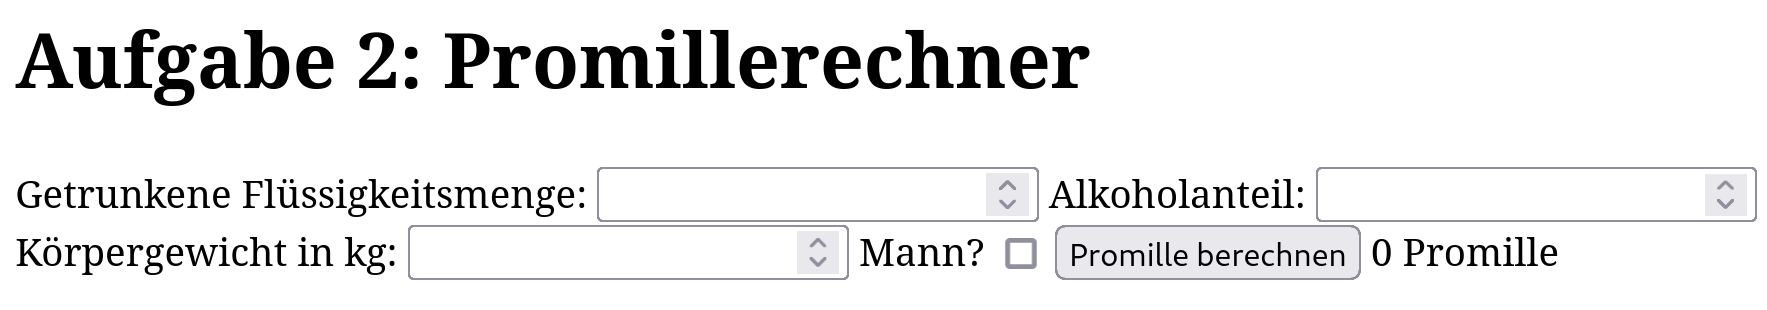
\includegraphics[width=\textwidth]{media/Promillerechner.png}
	\caption{Webseite des Promillerechners}
	\label{fig:promillerechner}
\end{figure}

Bei Nutzung der Webseite wurde demonstriert, dass diese keinerlei Funktion hatte.
Ein großes Ziel der ersten Doppelstunde war, den aktuellen Vorwissensstand der Schülerinnen und Schüler zum Thema Webentwicklung herauszufinden.
Die präsentierte Webseite wurde so einerseits dazu genutzt, um den Schülerinnen und Schüler einen Ausblick auf die kommenden Stunden zu geben und ihnen klar zu machen, dass wir uns nun (wieder) mit dem Thema Webentwicklung beschäftigen.
Andererseits wurde damit auch eine Diskussion darüber angestoßen, aus was eine Webseite denn besteht und woran sie sich noch erinnern können.
An dieser beteiligten sich die Schülerinnen und Schüler sehr engagiert und es fielen auch Fachbegriffe wie HTML.
Auf Nachfrage wurde jedoch schnell ersichtlich, dass nur wenig Wissen über das Thema HTML vorhanden war.

Dies wurde als Überleitung zum ersten Arbeitsblatt genutzt, welches in \autoref{pdf:AB_HTML_CSS} zu sehen ist.
Das Übungsblatt sollte zunächst in Einzelarbeit bearbeitet werden, bei Schwierigkeiten konnten die Schülerinnen und Schüler jedoch selbstständig zur Partnerarbeit übergehen.
In der Besprechung des Blatts wurde schnell klar, dass die meisten Fragen nur durch Internetrecherche beantwortet werden konnten und viele der Lerninhalte aus der Einheit zu HTML nicht mehr präsent waren.
Mit CSS konnte nur ein Schüler etwas anfangen, die anderen hatten noch nie davon gehört.
Während dies für die Schülerinnen und Schüler frustrierend gewirkt haben kann, war es dennoch ein wichtiges Vorgehen.
Nun war klar, dass die kommenden Stunden nicht auf Dinge aufbauen konnten, die über ein Grundwissen von HTML hinausgingen und kein bzw. nur sehr grundlegendes CSS verwendet werden konnte.

Die anschließende Erklärung der Syntax von Javascript und ihren Aufbau als Programmiersprache verlief grundsätzlich produktiv.
Von den Schülerinnen und Schülern kamen nur wenige Fragen, jedoch wurde anschließend das in \autoref{pdf:Merkblatt_Variablen_if} stehende Merkblatt als sehr hilfreich erachtet.
Lediglich die für die kommenden Aufgaben notwendige Funktion \texttt{document.getElementById()} war schwierig zu verstehen.
Hier konnte die Verwendung durch zahlreiche Beispiele anhand der Nutzung der Funktion in der Konsole auf einer Webseite verdeutlicht werden.
Dennoch sollte dies ein Problem bleiben, welches dauerhaft bestehen blieb, was sich jedoch erst beim Feedback am Ende der Unterrichtseinheit herausstellte.

Die oben genannten Schwierigkeiten spiegelten sich auch in der Bearbeitung des folgenden Übungsblattes wider, welches sich in \autoref{pdf:AB_Variablen_if} finden lässt.
Viele Schülerinnen und Schüler wussten nicht weiter.
Resultierend daraus mussten zusätzliche Erklärungen und Beispiele eingeschoben sowie die Bearbeitungszeit für das Blatt nach oben angepasst werden.


\subsection{Zweite Doppelstunde}
\label{subsec:doppelstunde-2}

\subsection{Dritte Doppelstunde}
\label{subsec:doppelstunde-3}

\subsection{Vierte Doppelstunde}
\label{subsec:doppelstunde-4}